\begin{abstract}
We propose Flow-GRPO, the first method to integrate online policy gradient reinforcement learning (RL) into flow matching models. Our approach uses two key strategies: (1) an ODE-to-SDE conversion that transforms a deterministic Ordinary Differential Equation (ODE) into an equivalent Stochastic Differential Equation (SDE) that matches the original model's marginal distribution at all timesteps, enabling statistical sampling for RL exploration; and (2) a Denoising Reduction strategy that reduces training denoising steps while retaining the original number of inference steps, significantly improving sampling efficiency without sacrificing performance.
Empirically, Flow-GRPO is effective across multiple text-to-image tasks. For compositional generation, RL-tuned SD3.5-M generates nearly perfect object counts, spatial relations, and fine-grained attributes, increasing GenEval accuracy from $63\%$ to $95\%$. In visual text rendering, accuracy improves from $59\%$ to $92\%$, greatly enhancing text generation. Flow-GRPO also achieves substantial gains in human preference alignment. Notably, very little reward hacking occurred, meaning rewards did not increase at the cost of appreciable image quality or diversity degradation.
% Project page: \url{https://flowgrpo.github.io}.
\end{abstract}

\definecolor{pltred}{HTML}{AF2519}
\definecolor{pltgreen}{HTML}{516E59}
\definecolor{pltblue}{HTML}{37527C}
\begin{figure}[ht]
\centering
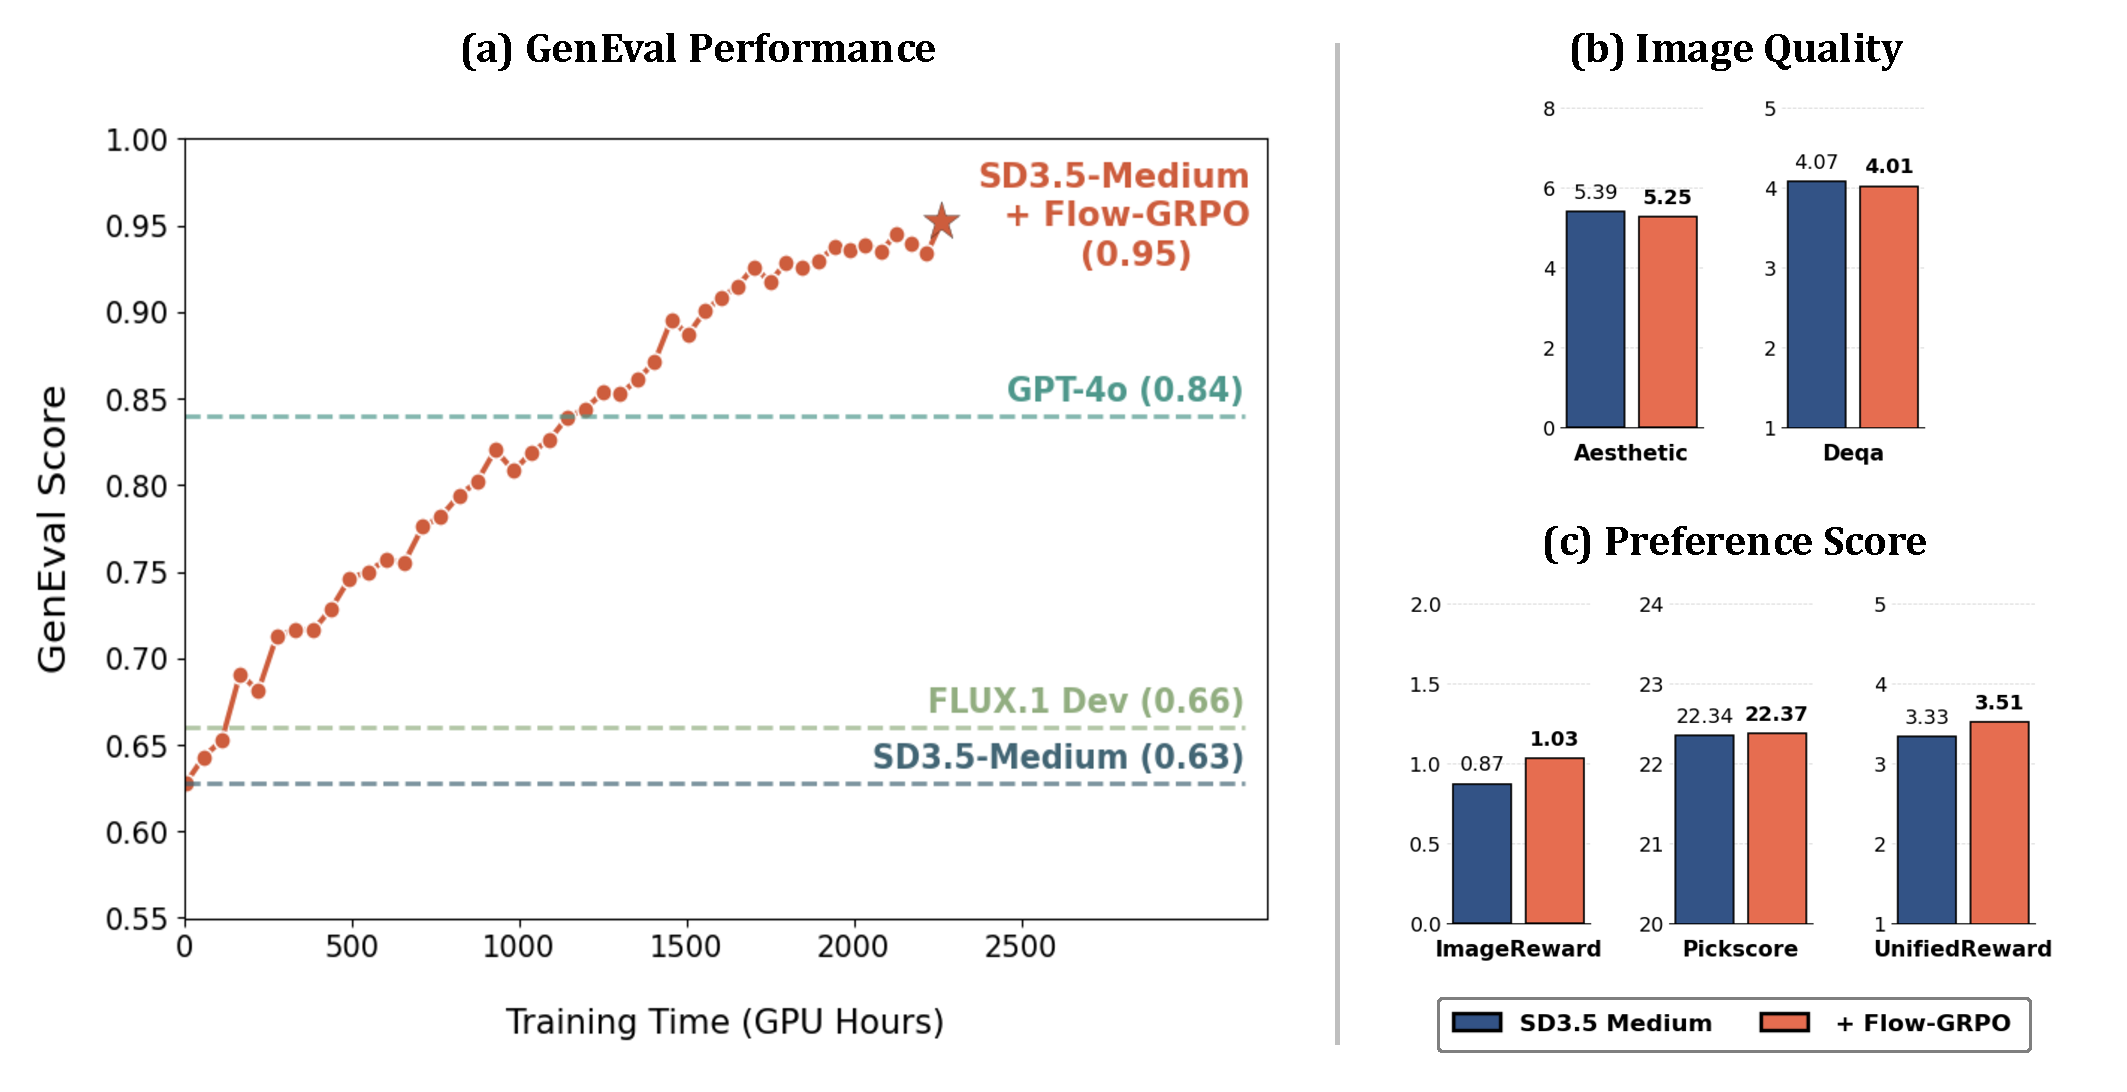
\includegraphics[width=\textwidth]{src/teaser.pdf}
\caption{ 
% \textcolor{pltred}{\textbf{(a) GenEval performance}} 
\textbf{(a) GenEval performance}
rises steadily throughout Flow-GRPO's training and outperforms GPT‑4o.
% \textcolor{pltgreen}{\textbf{(b) Image quality metrics}} 
\textbf{(b) Image quality metrics}
on DrawBench~\cite{drawbench} remain essentially unchanged.
% \textcolor{pltblue}{\textbf{(c) Human Preference Scores}} 
\textbf{(c) Human Preference Scores}
on DrawBench improves after training.
Results show that \emph{Flow-GRPO enhances the desired capability while preserving image quality and exhibiting minimal reward-hacking.}
}
\label{fig:teaser}
\vspace{-4mm}
\end{figure}